\section{Simulation}

\todo[inline]{TODO: Simulation...}
\todo[inline]{Napomenuti da se uzima u obzir dinamika aktuatora i rotora}
\todo[inline]{Napisati parametre letjelice}

\begin{figure}[h!]
	\centering
	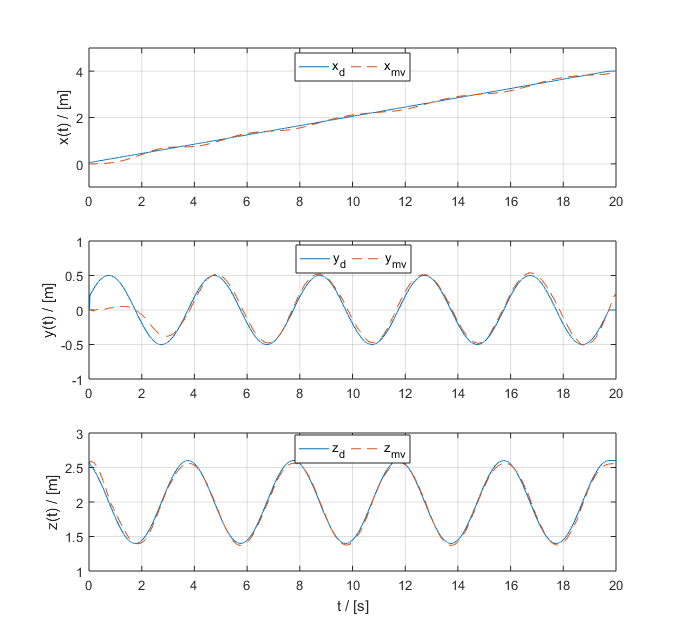
\includegraphics[width=\columnwidth]{./pictures/mmc_traj_pos.png}
	\caption{...}
	\label{fig:traj_pos}
\end{figure}

\begin{figure}[h!]
	\centering
	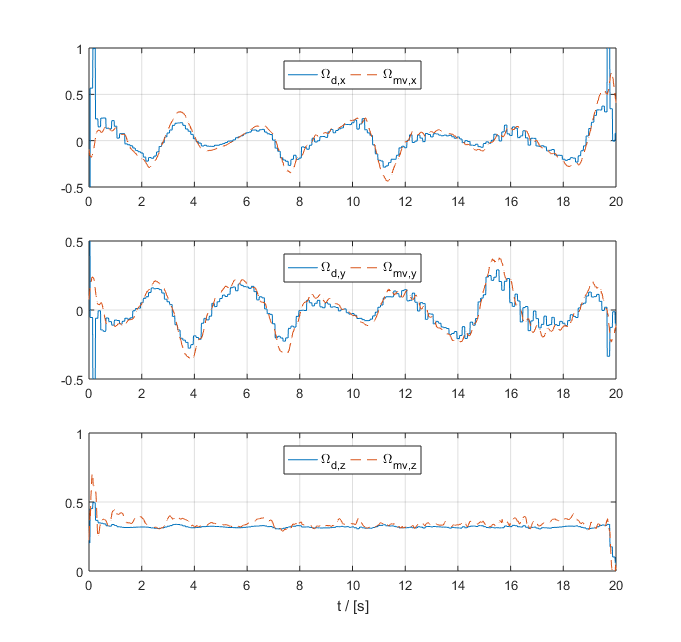
\includegraphics[width=\columnwidth]{./pictures/mmc_traj_omega.png}
	\caption{...}
	\label{fig:traj_omega}
\end{figure}

\begin{figure}[h!]
	\centering
	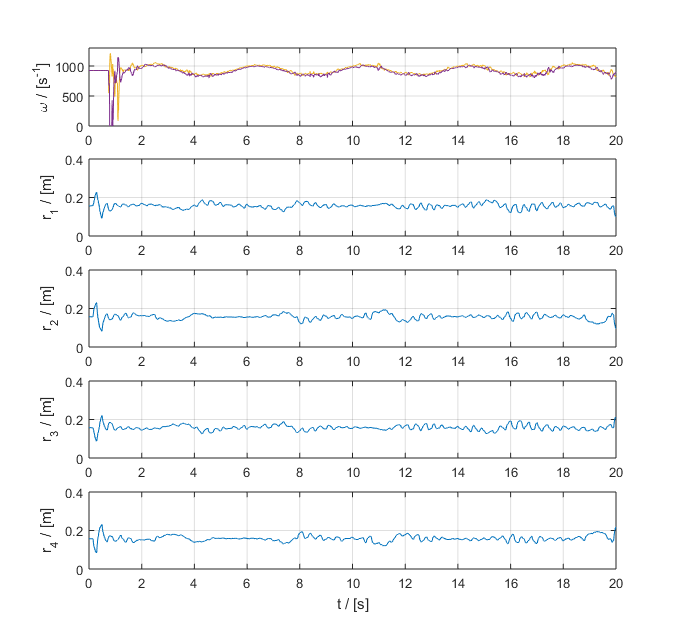
\includegraphics[width=\columnwidth]{./pictures/mmc_traj_rotorVel_massOff.png}
	\caption{...}
	\label{fig:rotorVel_massOff}
\end{figure}

\begin{figure}[h!]
	\centering
	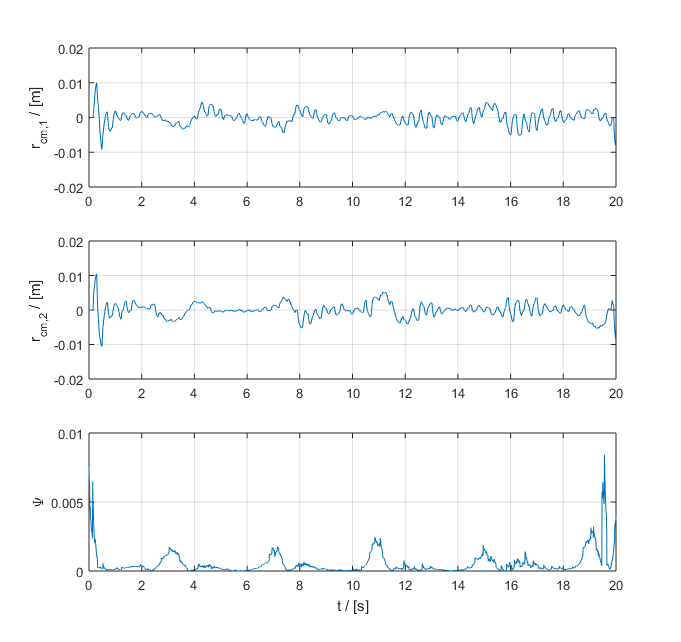
\includegraphics[width=\columnwidth]{./pictures/mmc_traj_rCm_attErr.png}
	\caption{...}
	\label{fig:rCm_attErr}
\end{figure}
